\documentclass[journal, a4paper]{IEEEtran}

% some very useful LaTeX packages include:

\usepackage{cite}      % Written by Donald Arseneau
                        % V1.6 and later of IEEEtran pre-defines the format
                        % of the cite.sty package \cite{} output to follow
                        % that of IEEE. Loading the cite package will
                        % result in citation numbers being automatically
                        % sorted and properly "ranged". i.e.,
                        % [1], [9], [2], [7], [5], [6]
                        % (without using cite.sty)
                        % will become:
                        % [1], [2], [5]--[7], [9] (using cite.sty)
                        % cite.sty's \cite will automatically add leading
                        % space, if needed. Use cite.sty's noadjust option
                        % (cite.sty V3.8 and later) if you want to turn this
                        % off. cite.sty is already installed on most LaTeX
                        % systems. The latest version can be obtained at:
                        % http://www.ctan.org/tex-archive/macros/latex/contrib/supported/cite/

\usepackage{graphicx}   % Written by David Carlisle and Sebastian Rahtz
                        % Required if you want graphics, photos, etc.
                        % graphicx.sty is already installed on most LaTeX
                        % systems. The latest version and documentation can
                        % be obtained at:
                        % http://www.ctan.org/tex-archive/macros/latex/required/graphics/
                        % Another good source of documentation is "Using
                        % Imported Graphics in LaTeX2e" by Keith Reckdahl
                        % which can be found as esplatex.ps and epslatex.pdf
                        % at: http://www.ctan.org/tex-archive/info/
\graphicspath{ {images/} }
\usepackage{tikz}
%\usepackage{psfrag}    % Written by Craig Barratt, Michael C. Grant,
                        % and David Carlisle
                        % This package allows you to substitute LaTeX
                        % commands for text in imported EPS graphic files.
                        % In this way, LaTeX symbols can be placed into
                        % graphics that have been generated by other
                        % applications. You must use latex->dvips->ps2pdf
                        % workflow (not direct pdf output from pdflatex) if
                        % you wish to use this capability because it works
                        % via some PostScript tricks. Alternatively, the
                        % graphics could be processed as separate files via
                        % psfrag and dvips, then converted to PDF for
                        % inclusion in the main file which uses pdflatex.
                        % Docs are in "The PSfrag System" by Michael C. Grant
                        % and David Carlisle. There is also some information
                        % about using psfrag in "Using Imported Graphics in
                        % LaTeX2e" by Keith Reckdahl which documents the
                        % graphicx package (see above). The psfrag package
                        % and documentation can be obtained at:
                        % http://www.ctan.org/tex-archive/macros/latex/contrib/supported/psfrag/

%\usepackage{subfigure} % Written by Steven Douglas Cochran
                        % This package makes it easy to put subfigures
                        % in your figures. i.e., "figure 1a and 1b"
                        % Docs are in "Using Imported Graphics in LaTeX2e"
                        % by Keith Reckdahl which also documents the graphicx
                        % package (see above). subfigure.sty is already
                        % installed on most LaTeX systems. The latest version
                        % and documentation can be obtained at:
                        % http://www.ctan.org/tex-archive/macros/latex/contrib/supported/subfigure/

\usepackage{url}        % Written by Donald Arseneau
                        % Provides better support for handling and breaking
                        % URLs. url.sty is already installed on most LaTeX
                        % systems. The latest version can be obtained at:
                        % http://www.ctan.org/tex-archive/macros/latex/contrib/other/misc/
                        % Read the url.sty source comments for usage information.
%\usepackage{stfloats}  % Written by Sigitas Tolusis
                        % Gives LaTeX2e the ability to do double column
                        % floats at the bottom of the page as well as the top.
                        % (e.g., "\begin{figure*}[!b]" is not normally
                        % possible in LaTeX2e). This is an invasive package
                        % which rewrites many portions of the LaTeX2e output
                        % routines. It may not work with other packages that
                        % modify the LaTeX2e output routine and/or with other
                        % versions of LaTeX. The latest version and
                        % documentation can be obtained at:
                        % http://www.ctan.org/tex-archive/macros/latex/contrib/supported/sttools/
                        % Documentation is contained in the stfloats.sty
                        % comments as well as in the presfull.pdf file.
                        % Do not use the stfloats baselinefloat ability as
                        % IEEE does not allow \baselineskip to stretch.
                        % Authors submitting work to the IEEE should note
                        % that IEEE rarely uses double column equations and
                        % that authors should try to avoid such use.
                        % Do not be tempted to use the cuted.sty or
                        % midfloat.sty package (by the same author) as IEEE
                        % does not format its papers in such ways.

\usepackage{amsmath}    % From the American Mathematical Society
                        % A popular package that provides many helpful commands
                        % for dealing with mathematics. Note that the AMSmath
                        % package sets \interdisplaylinepenalty to 10000 thus
                        % preventing page breaks from occurring within multiline
                        % equations. Use:
%\interdisplaylinepenalty=2500
                        % after loading amsmath to restore such page breaks
                        % as IEEEtran.cls normally does. amsmath.sty is already
                        % installed on most LaTeX systems. The latest version
                        % and documentation can be obtained at:
                        % http://www.ctan.org/tex-archive/macros/latex/required/amslatex/math/

\usepackage{gensymb}

% Other popular packages for formatting tables and equations include:

%\usepackage{array}
% Frank Mittelbach's and David Carlisle's array.sty which improves the
% LaTeX2e array and tabular environments to provide better appearances and
% additional user controls. array.sty is already installed on most systems.
% The latest version and documentation can be obtained at:
% http://www.ctan.org/tex-archive/macros/latex/required/tools/

% V1.6 of IEEEtran contains the IEEEeqnarray family of commands that can
% be used to generate multiline equations as well as matrices, tables, etc.

% Also of notable interest:
% Scott Pakin's eqparbox package for creating (automatically sized) equal
% width boxes. Available:
% http://www.ctan.org/tex-archive/macros/latex/contrib/supported/eqparbox/

% *** Do not adjust lengths that control margins, column widths, etc. ***
% *** Do not use packages that alter fonts (such as pslatex).         ***
% There should be no need to do such things with IEEEtran.cls V1.6 and later.
\usepackage{float}
\usepackage[justification=centering]{caption}

% Your document starts here!
\begin{document}

% Define document title and author
    \title{Beaver Works Summer Program Technical Report}
    \author{Michelle Tan}
    \maketitle

% Write abstract here
\begin{abstract}
    This material is part of a summer boot camp at MIT Beaver Works where teams of high schoolers program cars to compete in the Mini Grand Prix Challenge, an autonomous car race around a track. This four-week program meets on weekdays for eight hours each day. The program is based off the 6.141 Robotics Science and Systems class and the Robotics IAP at MIT. Each day typically consists of three lab periods, a technical lecture, a seminar with distinguished guest speakers, and an occasional communications class. 
\end{abstract}
% Each section begins with a \section{title} command
\section{Introduction}
    % \PARstart{}{} creates a tall first letter for this first paragraph
    \IEEEPARstart{T}{he} purpose of this program is to begin to understand the algorithms and methods used today in autonomous navigation and to experiment with them on a 1/10-scale racecar. Teams explore the abilities and limitations of building robust yet fast robotics systems through tasks such as following a wall, detecting a colored blob, following a colored blob, avoiding obstacles, using a color to decide whether to take a turn, and optionally implementing localization and mapping. Much of the class dealt with problems inherent to autonomous navigation, like sensor imperfections, accurate object detection from camera images, and speed constraints. 
    \par The cars used were referred to as RACECAR, which stands for Rapid Autonomous Complex-Environment Competing Ackermann-steering Robot. The cars were pre-built with its components prior to the start of the program, which include the NVIDIA quad-core CPU, a 192-core GPU, an Ackermann-steering system, and a large variety of sensors including a lidar(Light Detection And Ranging) sensor, camera, and odometer. The teams used ROS, a "meta" operating system for robots that focuses on modularity, interfaces, and code reuse. \cite{plecture2} 
% Main Part
\section{Week 1}
\subsection{Technical Goal}
In the first week, the learning objective was to get experience in working with the sensors and actuation of the robot and to also learn about control systems. The end-of-week challenge consisted of being able to follow a left and right wall at a desired distanced away at different starting positions from the wall. 
\subsection{Approach}
The teams were required to use lidar to sense the wall but they were free to implement a state controller of their choice. Several of the possible state controllers are described below. 
\subsubsection{Bang Bang Controller}The simplest of the controllers is the Bang Bang controller, which states that if the robot is too close, it should turn away and if too far, turn towards the wall. If the robot is the correct distance away, it goes straight. The Bang Bang controller uses a fixed speed and steering angle for each case, in contrast to the next kind of controller. 
\subsubsection{PID Controller}A more sophisticated method is to implement a PID controller which does calculations on the error values to determine an optimal steering angle to correct the robot's distance. The goal is for the robot to limit the amount of oscillations around the desired distance it takes until it is at the right distance. There are three parts to the PID controller: Proportional, Integral, and Derivative. They are incorporated in the equation below where u is the controller output and e is the error
\begin{equation}
u(t) = k_{p}e(t)+k_i\int_{0}^{t}e(\tau)d\tau + k_{d}e'(t)
\end{equation}
The proportional part allows the steering angle to scale linearly based on the error. The integral portion scales linearly with the total error over time. The derivative portion scales based on the derivative of the error in order to limit the overshoot. \cite{pid-mit}
\subsubsection{Two Point Controller}
When calculating the error distance, there was an additional consideration of which laser scan data to use. The angle of the robot could easily throw off the reading if only one measurement were taken, since the distance measured perpendicular from the robot will not necessarily be the true distance as shown below. \\ 
\begin{figure}[H]
\centering
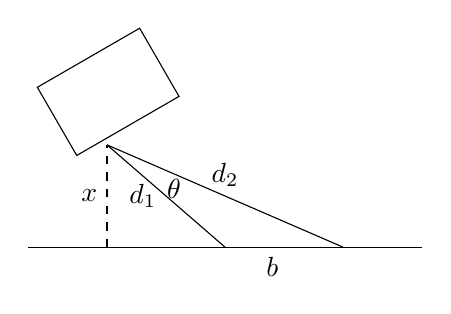
\begin{tikzpicture}
\draw[rotate around={30:(-1, 0.5)}] (0,3) rectangle(1.5,4);
\draw (-2,2)--(3,2) node at (1.1,2) [below] {$b$};
\draw [dashed] (-1,2)--(-1,3.3) node[midway, left]{$x$};
\draw (-1,3.3)--(0.5,2) node[midway, left]{$d_1$};
\draw (-1,3.3)--(2,2) node[midway, above]{$d_2$};
\draw node at (-0.15,2.5) [above] {$\theta$};
\end{tikzpicture}
\caption{Diagram of angled robot}
\end{figure}
A two point controller could account for this by using basic trigonometry to determine the true distance from the wall. Given two laser measurements $d_1$ and $d_2$ with a known $\theta$ between them, the following formula can calculate the true distance x between the wall and the robot.  
\begin{equation}
x = \frac{d_1d_2sin(\theta)}{\sqrt{d_1^2+d_2^2-2d_1d_2cos(\theta)}}
\end{equation}
\par Since there were so many options and there was not enough time to test all of them, we wrote code implementation of all of the separate features, like the PID controller and error calculation, so we could test each systematically to find the best option. We also decided to approach the challenge by starting simple and incrementally improving it.
\subsection{Process}
We decided to approach the challenge by starting with the simplest option and incrementally improving it.
\subsubsection{Error calculation}To calculate error, we decided to find the true distance to the wall by finding the minimum point in a range of laser distances. Mathematically, the true perpendicular distance is the shortest distance. This assumes that the robot is rotated such that the minimum distance is in the range of laser values taken. Given the parameters of the wall follow challenge, we thought this was a safe assumption. The points taken from the laser were in the range starting from 2.5\degree behind the robot to 5\degree  ahead of the robot.
\subsubsection{Bang Bang controller} After we could find the error, we started with the bang bang controller. This simple implementation was able to reliably follow a wall, even if the wall was curved. The problem with the Bang Bang control was when we started the robot far away from the line. Since the turning rate was independent from the actual distance from the wall, when the robot was far away, it would turn at a slower rate than it intuitively should given the distance away. Even worse was that when the robot was close to the desired distance, it would continue to use too steep of a steering angle, resulting in perpetual oscillations and jerkiness. 
\subsubsection{P Controller}We next tried implementing a P controller in order to control the steering angle more. In a P controller, the error is proportionally scaled to be the steering angle, so bigger error would result in more severe turning and on the other hand, smaller error would result in a more subtle turn. Higher $k_p$ values, would result in more responsiveness but also more unnecessary oscillations. We found that $k_p$ values near 1.0 achieved the best balance of reactiveness but not overreaction. The P controller was significantly better at correcting for large errors, but at very high distances, it would sometimes turn back so quickly that it would smash into the wall. 
\subsubsection{PD Controller}Afterwards, we tried moving to a PD controller. The Derivative portion would calculate the rate of change of the error and limit the change in order to attempt to smooth out the oscillations. After a lot of tuning of both  constants, we found that the derivative caused jerkiness no matter what value we had it at. This was most likely the result of noise. Although it was jerky we also found that it was  necessary for adjusting the distance when the robot was really far. 
\subsubsection{Final implementation}In the end, a large majority of the challenge had to do with finding the right constants. We were not able to find working constants for the entire PID controller due to lack of time, so we used a PD controller for the race. The setup that ended up working well was with a $k_p$ of 1, a $k_d$ of .05, and a $k_i$ of 0. 
With more time, we could have continued perfecting the numbers, but they were sufficient for this challenge. 

\subsection{Results}
The challenge consisted of a straight left and right wall that the robot should be able to follow. Three time trials were recorded on the different sides starting the robot at different distances. Then a challenge test was tried where the robot was put in the center of the 2-lane track, requiring agile recovery to avoid crashing into the wall. Every group was able to follow the wall, but few teams were able to correct the distance from the center of the track. 
\par We learned that although there is a lot of theoretical research on optimal values for the PID controller, what happens in real life is vastly different. The amount of time needed for testing is significantly higher than the time needed to write the code. We found that what should happen or what happens in simulation is not a substitute for real life testing. Our car was able to complete the race with the following scores: \\
    \begin{table}[!hbt]
        % Center the table
        \begin{center}
        % Title of the table
        \caption{Final Challenge times}
        % Table itself: here we have two columns which are centered and have lines to the left, right and in the middle: |c|c|
        \begin{tabular}{|c|c|}
            % To create a horizontal line, type \hline
            \hline
            % To end a column type &
            % For a linebreak type \\
            Left Wall & 8.77 \\
            \hline
            Right Wall & 8.85 \\
            \hline
        \end{tabular}
        \end{center}
    \end{table} \\
Although we were 8th out of 9 teams, the times were all within .2 seconds of each other so external factors from our algorithm such as battery level or timer inaccuracy could also have an effect. With more time, the constants could have been tuned to more optimal values and to also include a $k_i$ value.
\section{Week 2}
\subsection{Technical goals}
The challenge from this week was to use the ZED camera to sense a colored blob and use visual servoing to follow the blob. When the car was close enough, the robot had to make a correct turn based on the color of the blob where green indicated a right turn and red indicated a left turn. Afterwards, the program had to successfully wall follow until a certain point. The following diagram is taken from the lab handout for the week 2 challenge. \\ 
\begin{figure}[H]
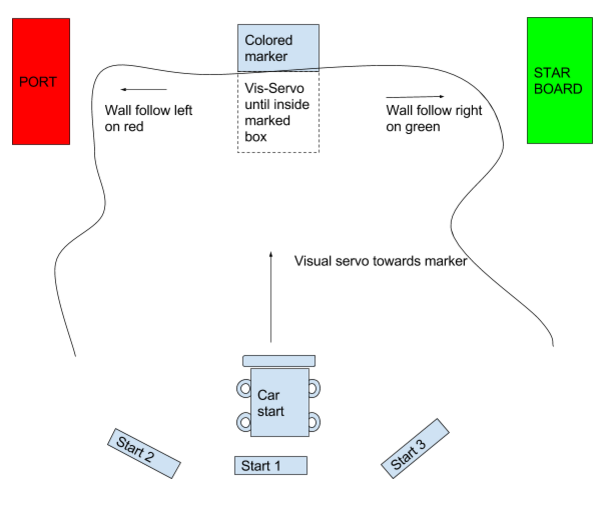
\includegraphics[scale=.42]{visual_servo.png}
\caption{Challenge diagram \cite{vs-handout}} 
\end{figure}
\subsection{Approach}
We started with getting a good blob detections algorithm. Then we came up with a simple but effective algorithm to have the robot drive towards the blob. It would then have to turn 90 \degree before transitioning into the wall following program from last week. We split up the task into a blob detections node, a blob follow node and a wall follow node in order to facilitate testing and so we could split up the work effectively. 
\subsection{Process}
\subsubsection{Blob Detections}We first focused on being able to detect a colored blob using the OpenCV library. In a lab session, we worked individually on each getting good blob detection. Everyone in the team put the working parts of their code together and we built off the final one. There were many possible approaches to find blobs such as finding contiguous colors and edge detection, but we decided to detect contours. According to OpenCV documentation, contours are "a curve joining all the continuous points (along the boundary), having same color or intensity." \cite{opencv-docs} The first step was to convert the image from RGB(Red-Green-Blue) to HSV(Hue-Saturation-Value). HSV is a color space that is convenient for processing colors in real-life images because it accounts for different lightings of an object as being of the same color. \cite{colorspace-handout} We first use masks to filter for the desired color and changed the image to gray scale in order to make the contours more accurate. After drawing the contours, it would check if the size is larger than a certain threshold in order to eliminate noise. If the program determined that it was a blob, it would publish the detections to a separate node using a custom message. 
\subsubsection{Visual servo}While part of the team was working on publishing blob detections, others worked on visual servoing. The simplest algorithm was a bang bang controller based on height and x position of the blob. If the blob was too short that meant it was too far so it would go forwards. If the blob was too tall, it meant that it was close enough and the robot would stop. If the x position of the blob was on the right side of the screen, the robot turned right to orient with the blob. Likewise, if the x position of the blob was on the left side, the robot turned left. As expected with a bang bang controller, it was jerky and when we were close to the target, it had trouble getting oriented because if it was a little off center, it would turn back too much and be stuck in an oscillation cycle. We decided to implement a PID controller into our visual servo, which helped with this issue. 
\subsubsection{Wall Follow}We also had to modify our wall-follow code from last week and optimize it for our situation. We did not focus on tuning this part too much because we knew it functioned from last week. Most of the work was integrating it to work with the other nodes.
\subsubsection{Node communication}This week, the structure of the task and how the nodes would communicate was essential to getting a working program. We had a blob detection node that would publish a custom blob message onto a visual servo node, which would then move towards the blob. When this node was finished, it had to send exactly one message to the wall follow node indicating whether to take a left or right turn. Eventually, we were able to successfully integrate them together. Due to miscommunication, we realized that no one had programmed the turn for when it got to the wall. We struggled to get that part working for the race because of lack of testing time. 
\subsection{Results}
At the very last minute we were able to get the robot to turn and follow properly when it got to the wall. Unfortunately, it only worked on the green side because we figured out later that there was a bug in our code where the isGreen variable we were modifying was a local variable so it was not stored between functions. Then during the race, our robot did not move probably due to lack of battery. After we charged it, the program did not work the same way and the gears had a glitch, so unfortunately we could not finish in the actual race. Out of all of the teams, only 2 were able to finish. We learned important lessons in communicating to make sure everything is getting done and to make sure the robot is charging. 
\section{Week 3}
\subsection{Technical goals}
This week, the focus was on how to get around a track and how to avoid obstacles. Our final challenge was to use reactive-based planning based on lidar in order to explore unbounded space while avoiding obstacles. We also had to detect blobs along the way and save the picture with the blob color and locations indicated. To add on from the image detection from last week, additional colors to detect were added(blue and yellow), and there was a challenge task to detect images of Ari, Sertac, a cat, and a robot. 
\subsection{Approach}
Based on the open-ended nature of this week's assignment, we had a team meeting where we discussed a lot of possible methods for obstacle avoidance and ways to conditionally take a shortcut. We first focused on ways to get around without obstacles. We had different people explore different ideas. In the end, we ended up using a potential field method that we learned about in a lecture, which was the most effective.
\subsection{Process}
Here are some of the methods we explored
\subsubsection{Right wall follow}
If there are no obstacles and we are not supposed to take the shortcut, we thought that a simple wall follow should be sufficient. However, we found that because of the sharp corner, it would not be an option. As the robot approached the corner, it could never determine that it should turn until it had already run into the wall, since the robot looks out to the side and not directly in front of it. After we adjusted the field of vision to angles further up front, it was able to turn at the corner only at very low speeds. 
\subsubsection{Equal Distance wall following}
Assuming there are no obstacles, an effective way to take the shortcut would be to simply follow the wall on both sides by trying to keep the distances on the left and the right the same. When the robot got to the shortcut, it would see a large spike in the laser reading for the left side and therefore turn left to account for it. However, it was determined that this model would break down with obstacles. 
\subsubsection{Obstacle detect}
The robot would look ahead and if obstacles are detected on the left side, it would take the right lane and vice versa. If both left lane and right lane have obstacles, then it would take the center lane. The idea of changing the desired distance of the wall follow based on where the obstacles are is valid, but too many assumptions were made in the model like how the object had to be in either the left, middle, or right. 
\subsubsection{Left/Right Wall Follow}
If there are no obstacles, follow the left wall the whole time, then switch to following the right wall when there is the shortcut to ensure that the robot takes the long way around.
\subsubsection{State machine}
We explored enough options for the cases of wanting to take the shortcut and not taking the shortcut, along with how to avoid obstacles, that we could incorporate them all into a state machine. It would perform some sort of wall follow as a default, but if obstacles are detected, the obstacle avoidance program would take precedence. 
\subsubsection{Open space}
Use the lidar to find the largest contiguous open space and go there. This method could work well, especially for avoiding obstacles. We ran out of testing time to try it out, however. 
\subsubsection{Potential field}
The potential field method uses the idea of charges attracting and repelling to control the robot. The robot is repelled from obstacles, but also repelled from behind so it continues to move forwards. We ended up using this method because it was the most robust to all of the possible scenarios. This implementation was the most effective and also the most simple at under 20 lines of code. 

\subsubsection{Challenge blob detection} For the blob detections, we used the version we made last week and added in the new colors. We came up with two possible solutions that we could have had working with more time. The first one was to average the HSV values of the pixels in each of the challenge images and hope that they are different enough that we could distinguish them. This would be messed up in different lightings, but since we are not penalized for incorrect labeling, we thought it could be worth it. The second method would be to do some sort of statistical analysis of the HSV values of the pixels of the original images. Then, we could find the distribution for the blobs from the ZED camera and compare them to find the closest match. This process was simplified because we found cv2 functions for calculating and comparing histograms. Since this method seemed more robust to lighting changes and distortions, we started implementing this method. 
\subsection{Results}
In the final challenge, we used the potential field method. We ran out of time to execute the challenge images and we were not able to tune the color values well, so we missed a lot of colors in the actual challenge. We should have spent more time tuning the colors instead of focusing on the challenge images since in the end, none of the teams could detect the challenge images. We ended up coming in 3rd place with 36 points, which came from detecting four blobs and having two collisions. 

\section{Week 4}
\subsection{Technical goals}
This week was dedicated to preparation for the Grand Prix Challenge race, but in addition there were two tech challenges that would be informally showcased. 
\subsubsection{Tech Challenge 1}
In the first tech challenge, the robot had to publish blob detections while it explored an unstructured space with obstacles. This was very similar to the task from week 3.
\subsubsection{Tech Challenge 2}
In the second tech challenge, the robot had to go along the racetrack and look for a colored blob that would be located at a forked intersection. A green blob would indicate an open shortcut that the robot could take while a red blob would indicate that the shortcut was blocked and the robot had to take a longer way around. \\ 
\subsubsection{Grand Prix Race}
The Grand Prix Race is the culmination of all of our work done thus far in the summer. The cars were supposed to race around the track, avoiding nearby cars. In addition, at one point in the track there was a fork with two different paths: a straight shortcut and a longer path curving on the right side. Based on the color of a blob placed in the intersection, the car would have to determine if the shortcut was open given that a red blob indicated a blocked shortcut. 
\begin{figure}[H]
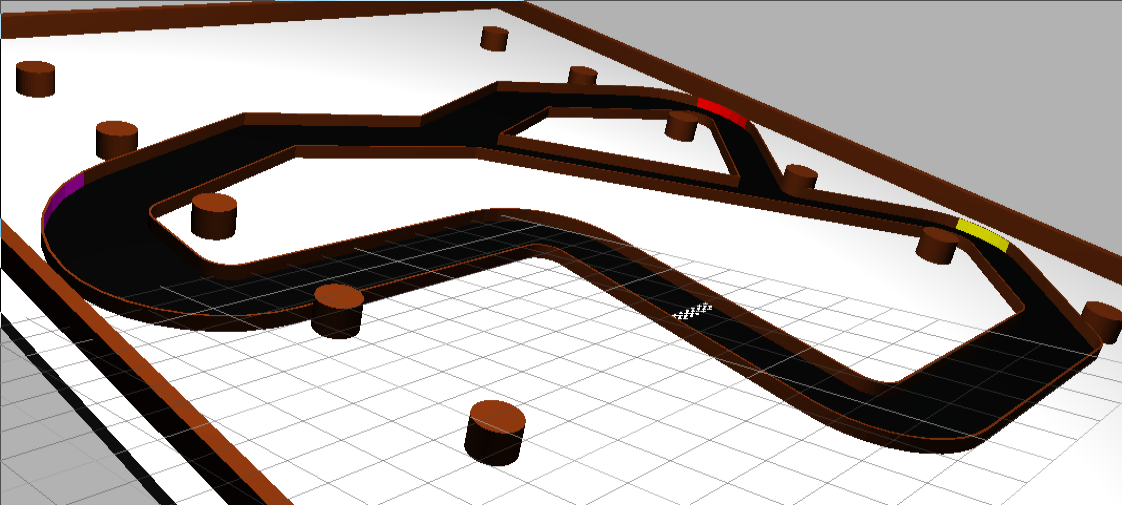
\includegraphics[scale=.20]{gazebo_track.png}
\caption{Model of racetrack \cite{gazebo_pic}} 
\end{figure}
\subsection{Approach}
Since this Grand Prix was the only task that was scored, we wanted to focus on that task and make sure we had enough time to test it. In addition, the 2nd tech challenge is part of the Grand Prix challenge so it would not require extra work if the the Grand Prix code worked. Any extra time we had would be spent working on the 1st tech challenge. Since we would be switching locations to the Walker Memorial which has different lighting and is also prone to further lighting changes due to natural light, we tried to speed up the process of fine-tuning the HSV values using a calibration program.
\subsection{Process}
\subsubsection{Detecting blobs and exploring space}
This challenge builds on the program we had last week for reactive planning, which was able to detect red, yellow, green, blue, and pink blobs. We wanted to continue testing and improving on the challenge images implementation from last week. In addition, the colored blobs could also be circles, rhombi, x shapes, and plus signs so the program had to distinguish between them. We found that a quick way to distinguish between them would be to inscribe each shape in a rectangle and compare the ratios of the area of the shape to the area of the rectangle. \\
\begin{figure}[H]
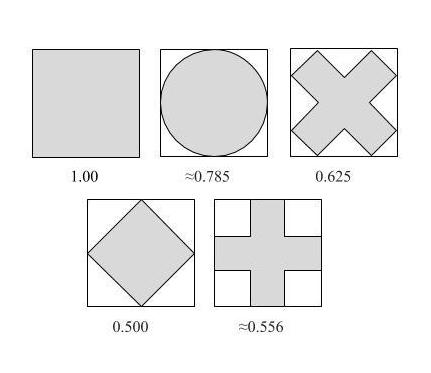
\includegraphics[scale=.50]{ratios.jpg}
\caption{Shows the ratio of the area of the inscribed shape to the square} 
\end{figure}
As shown above, the ratios are all different, but some may be close enough with each other to get confused. We only had time to implement a simple algorithm like this one. 
\subsubsection{Navigating around the track}
We decided to try modifying the reactive obstacle detection program from last week that used potential fields to guide the robot away from obstacles. This program was the most robust to being able to deal with all different kinds of obstacle configurations. The only modification that seemed to be needed was a larger imaginary charge behind the robot so it was not tempted to go backwards. In addition, we noticed that the track contained 4 major left turns and 2 major right turns(one of these being the intersection). When on a left turn, the most efficient path would be to stick to the left wall more, minimizing the distance. Since all of the cars have the same maximum speed, we realized that we could get an edge by staying on the inside lane. We implemented this by adding a boost constant to the force to the left when calculating the vector of least resistance. This required a lot of tuning to ensure that it would favor the left while not crashing into it. 
\subsubsection{Detecting shortcut availability}
Instead of calibrating the robot to look for red or green, the robot looked for only red. If there was red detected, it would take the long way. Otherwise, it would assume that the shortcut is open. In order to make the right turn successfully we had to modify the forces on the robot to make it favor the right side. We had a problem with as the robot was turning, when it lost sight of the red blob it would stop turning. In addition, the left wall affinity would cause the robot to veer left so aggresively after turning that it would crash into the wall. We had to set up a counter that would execute as soon as it saw the red blob. For the first part of the counter, it would highly favor right turning until it had basically finished the turn. For the second part of the counter, it would switch lanes to the center to ease the transition to the left wall. Then, lastly the default track navigation code would continue as normal. 
\subsubsection{Color calibration}
Since there seemed to be a problem with color thresholds changing with different lightings, we made a calibration program that would use the ZED Camera to take a picture of the blob. Then, we could analyze the distributions of the H,S, and V values using a histogram. The following are the histograms from data taken on August 3rd. \\
\begin{figure}[H]
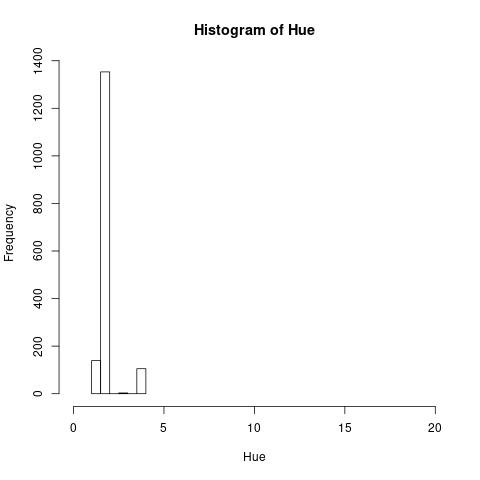
\includegraphics[scale=.50]{hplot.jpg}
\caption{Distribution of the Hues: Values range from 0 to 5}
\end{figure}
\begin{figure}[H]
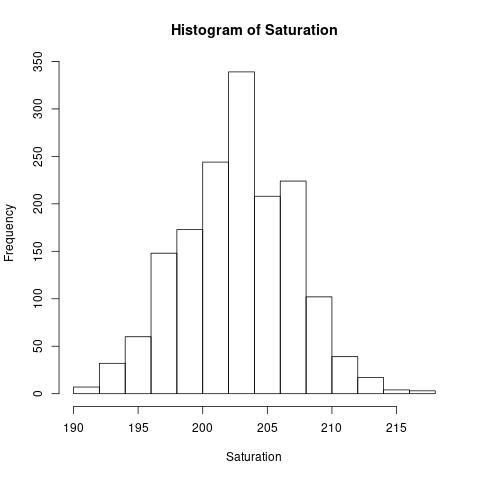
\includegraphics[scale=.50]{splot.jpg}
\caption{Distribution of the Saturation: Values range from 190 to 220}
\end{figure}
\begin{figure}[H]
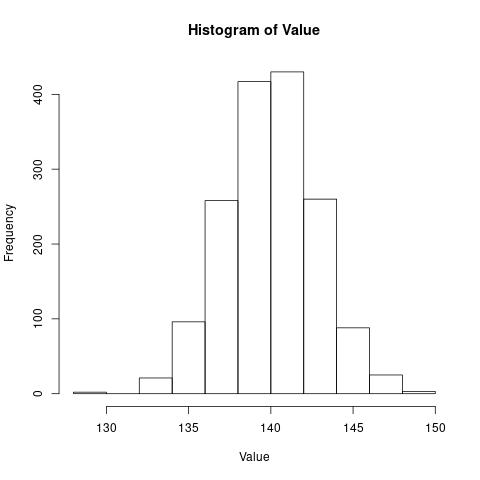
\includegraphics[scale=.50]{vplot.jpg}
\caption{Distribution of the Values: Values range from 125 to 150}
\end{figure}
Based on this data, we had an estimate of what we should set the HSV values to. However, we widened the threshold past what the histogram showed because the pictures for the data were taken under ideal situations. In reality, the colors would be affected by shadows of people and distance away from the blob. In this case, it was preferable to widen the range to the maximum values that would not start picking up other objects as the blob, since our issue was that it was missing the red blob. We ended up using the values shown below \\
    \begin{table}[!hbt]
        % Center the table
        \begin{center}
        % Title of the table
        \caption{HSV values for red}
        % Table itself: here we have two columns which are centered and have lines to the left, right and in the middle: |c|c|
        \begin{tabular}{|c|c|c|c|}
            % To create a horizontal line, type \hline
            \hline
            % To end a column type &
            % For a linebreak type \\
              & Hue & Saturation & Value\\
            \hline
            Lower Bound& 0 & 150 & 80 \\
            \hline
            Upper Bound & 6 & 255 & 255 \\
            \hline
        \end{tabular}
        \end{center}
    \end{table} \\

\subsection{Results}
\subsubsection{Tech Challenge 1}
Our robot was able to navigate while avoiding obstacles. It was able to detect colored blobs, but unfortunately we did not put enough time into testing to have it reliably detect the challenge images or the alternate shapes.
\subsubsection{Grand Prix Race}
Our team did really well. We were ranked 1st out of all 9 teams in both the time trials with the following times:
    \begin{table}[!hbt]
        % Center the table
        \begin{center}
        % Title of the table
        \caption{Time Trial Results}
        % Table itself: here we have two columns which are centered and have lines to the left, right and in the middle: |c|c|
        \begin{tabular}{|c|c|c|}
            % To create a horizontal line, type \hline
            \hline
            % To end a column type &
            % For a linebreak type \\
			\textbf{Lap \#} & \textbf{Color of blob} & \textbf{Time} \\
			\hline
            1 & Green & 28.93\\
            \hline
            2 & Red & 33.46 \\
            \hline
            3 & Red & 33.28\\
            \hline
        \end{tabular}
        \end{center}
    \end{table}
    \begin{table}[!hbt]
        % Center the table
        \begin{center}
        % Title of the table
		\caption{Final Grand Prix Results}
        % Table itself: here we have two columns which are centered and have lines to the left, right and in the middle: |c|c|
        \begin{tabular}{|c|c|}
            % To create a horizontal line, type \hline
            \hline
            % To end a column type &
            % For a linebreak type \\
			\textbf{Color} & \textbf{Time} \\
			\hline
            Green & 28.00 \\
            \hline
            Red & 38.20 \\
            \hline
        \end{tabular}
        \end{center}
    \end{table}
\section{Conclusion}
\par The goals in this summer program were to learn about autonomous navigation, sensors, state controllers, object detection, object avoidance, and SLAM(Simultaneous Localization and Mapping). We managed to explore all of these topics expect for Localization and Mapping. The lidar's data was not detailed enough to be able to get a reasonably accurate map of the track with the obstacles. The results were an autonomous robot that could detect colored blobs, follow a wall, avoid obstacles, and follow a track. 
\par I learned about ROS and how the structure of modular programming allows for greater complexity. I also learned about the different controllers that could be implemented and the advantages of closed loop control over open loop control. We learned about methods used for detecting colored objects which included looking for contours and edges of a certain size and color. We also learned how to apply the concept of potential field to make a robot that avoided obstacles. 

\par Going forward, I will remember the importance of leaving enough time to test and how to stick to a list of priorities. In addition, the ability to collaborate effectively was essential to our final success. 

\nocite{5}
% Now we need a bibliography:
\bibliographystyle{unsrt}
\bibliography{report}

% Your document ends here!
\end{document}
